\chapter{相变}\label{ch:b3:phase-transitions}

将水加热一度，几乎毫无变化——直到
在某一定义十分清晰的温度，液体骤然化为蒸气。
将铁冷却并穿越 \qty{1043}{K}，成分不变，
它便自发磁化。单个分子或单个自旋中看不出
这些转变的迹象：它们是\emph{集体}行为
——$10^{23}$ 个个体，各自仅与少数近邻相互作用，
却同时改变整个体系的相态。本科一年级
分册已对各类转变作了归类；本章则阐明其
机制，借助最近五章的工具：自由能竞争、
序参量、对称性破缺，以及一个令人惊讶的
发现：在临界点附近，微观细节
不再重要——磁体与沸腾流体具有相同的
临界指数。本章的思想，从高压锅
到超导体，直至
\cref{ch:b3:particle-physics}中的希格斯场。

\section{序参量与自由能竞争}

\begin{definition}[相与序参量]\label{def:b3:phase-transitions:order}
\index{相变}\index{序参量}\index{对称性破缺}
称\emph{相变}为系统平衡态的一种非光滑变化，
即控制参量（$T$、$P$、$B$）穿越某一边界时
的平衡态随之改变。其度量为\emph{序参量}：在无序相中为零、
在有序相中非零的量——例如
铁磁体的磁化强度 $m$，流体的密度差
$\rho_{\text{液}} - \rho_{\text{气}}$，以及
\cref{ch:b3:quantum-statistics}中的凝聚份额。相变
分两类：\emph{一级相变}（序参量跳变；有潜热；
两相共存——如沸腾、熔化），以及\emph{连续相变}（序参量
自零连续增长；无潜热；涨落剧烈——如
居里点、临界点与超流氦）。有序态若必须
在若干等价选项中\emph{选择}——例如磁体的北极
必须指向某一方向，相变便发生
\emph{对称性破缺}，即破坏了基本定律所遵从的一种对称性；
这一主题将在最高层次上随希格斯机制再次出现。
每种情形背后的驱动力都是自由能 $F = E - TS$
（\cref{prop:b3:canonical-ensemble:machine}）：能量偏向有序，
熵偏向无序，$T$ 决定两者的兑换比率——相界
正是两者恰好相抵之处。
\end{definition}

\section{液–气相变：范德瓦耳斯}

\begin{proposition}[范德瓦耳斯等温线]\label{prop:b3:phase-transitions:vdw}
\index{范德瓦耳斯方程}\index{临界点}
本科一年级分册中的真实气体方程，
\[
\Big(P + \frac{aN^2}{V^2}\Big)(V - Nb) = Nk_{\text{B}}T ,
\]
它体现了分子间吸引（$a$）与硬核（$b$）。高于临界
温度 $T_{\text{c}} = 8a/27bk_{\text{B}}$ 时，等温线
单调：只有一个流体相。低于该温度时，等温线形成一个环，其中含有
力学上\emph{不稳定}的一段（$\partial P/\partial V >
0$）：该段流体分裂为共存的液相与气相，
压强由化学势相等所确定（麦克斯韦
等面积法则）。共存区于临界
点闭合，即（$P_{\text{c}}, V_{\text{c}}, T_{\text{c}}$）处，液相与气相
变得\emph{不可区分}：趋近该点时，
密度差趋于零，压缩率发散，
密度涨落增长至可见光尺度——即
临界乳光（见\cref{pb:b3:perturbation-theory:1}）。
\end{proposition}
\admitted

\begin{omfigure}
\begin{tikzpicture}
  \begin{axis}[omaxis, axis x line=bottom, axis y line=left,
    width=10.8cm, height=6.0cm, xmin=0.32, xmax=5, ymin=0, ymax=2.1,
    xlabel={$V/V_{\text{c}}$}, ylabel={$P/P_{\text{c}}$},
    xlabel style={at={(axis description cs:0.5,-0.09)}, anchor=north},
    xtick={1,2,3,4}, ytick={1}, clip=true,
    legend pos=north east,
    legend style={font=\scriptsize, draw=none, fill=none}]
    % reduced vdw: P = 8T/(3V-1) - 3/V^2 (T in units of Tc)
    \addplot[omDef, very thick, domain=0.42:5, samples=250]
      {8*1.05/(3*x-1) - 3/(x*x)};
    \addplot[omThm, very thick, domain=0.42:5, samples=250]
      {8/(3*x-1) - 3/(x*x)};
    \addplot[omExo, very thick, domain=0.44:5, samples=300]
      {8*0.9/(3*x-1) - 3/(x*x)};
    \legend{$T > T_{\text{c}}$, $T = T_{\text{c}}$, $T < T_{\text{c}}$}
    % coexistence dome (schematic)
    \addplot[gray, dashed, domain=0.5:2.9, samples=100, forget plot]
      {1 - 0.62*(ln(x/1.06))^2};
    \fill (axis cs:1,1) circle (1.8pt);
    \draw[gray, ->] (axis cs:1.55,1.5) -- (axis cs:1.05,1.06);
    \node[font=\scriptsize, anchor=west] at (axis cs:1.6,1.55)
      {临界点};
    \node[gray, font=\scriptsize, anchor=north] at (axis cs:1.7,0.62)
      {共存穹顶};
  \end{axis}
\end{tikzpicture}

{\small 约化单位下的范德瓦耳斯等温线。高于
$T_{\text{c}}$：单一流体。低于该温度时，环的不稳定中段
被虚线穹顶内的平坦两相共存所取代。于
穹顶顶点处，液相与气相合并——即临界点，
涨落使流体变得浑浊。}
\end{omfigure}

\begin{proposition}[克劳修斯–克拉珀龙]\label{prop:b3:phase-transitions:clapeyron}
\index{克劳修斯–克拉珀龙关系}
沿任一一级共存线，两侧化学
势相等，
由（见\cref{def:b3:grand-canonical:mu}）可知，该线的斜率必为
\[
\frac{\dd P}{\dd T} = \frac{L}{T\,\Delta v} ,
\]
其中 $L$ 为潜热，$\Delta v$ 为每个
粒子（或每千克，二者须统一）。共存线的一切
信息均蕴含于此式：水的沸腾线
在 \qty{100}{\celsius} 附近以 $\approx\qty{3.6}{kPa/K}$ 的斜率上升，
（高压锅、高海拔烹饪——见
\cref{pb:b3:phase-transitions:1}）；而水的\emph{熔化}线
向后倾斜（$\Delta v < 0$：冰会漂浮），因此压力可使
冰熔化——这在多数物质中十分罕见，其影响从冰川
延伸至溜冰场。
\end{proposition}

\begin{proof}
在该曲线上 $\mu_1(T, P) = \mu_2(T, P)$；沿曲线移动：
$-s_1\dd T + v_1\dd P = -s_2\dd T + v_2\dd P$（每个粒子，利用
$\dd\mu = -s\,\dd T + v\,\dd P$）。解出 $\dd P/\dd T$，并利用
$L = T(s_2 - s_1)$。
\end{proof}

\section{铁磁体：平均场理论}

\begin{theorem}[平均场伊辛相变]\label{thm:b3:phase-transitions:meanfield}
\index{伊辛模型}\index{平均场理论}\index{居里温度}
将磁铁建模为格点上的自旋 $s_i = \pm1$，近邻之间
通过交换能 $-J\,s_is_j$ 耦合
（见\cref{exo:b3:identical-particles:12}），每个自旋有 $q$
个近邻。以近邻的平均值 $m =
\langle s\rangle$ 代替其近邻（即\emph{平均场}近似）；
此时每个自旋处于有效场 $qJm$ 中，由
\cref{exo:b3:canonical-ensemble:11} 可得
自洽条件
\[
m = \tanh\!\Big(\frac{T_{\text{c}}}{T}\,m\Big) , \qquad
k_{\text{B}}T_{\text{c}} = qJ .
\]
在 $T_{\text{c}}$ 以上，唯一解为 $m = 0$；
在其以下，出现两个对称解 $\pm m(T)$，二者均稳定：
磁铁\emph{必然}磁化，并随机选取一个方向——
即自发对称性破缺。在 $T_{\text{c}}$ 附近，$m \propto
(T_{\text{c}} - T)^{1/2}$；在其以上，磁化率服从
居里–外斯定律 $\chi \propto 1/(T - T_{\text{c}})$：
在相变点发散——一块无限“听话”的磁铁。
\end{theorem}

\begin{proof}[部分证明]
处于场 $B_{\text{eff}} = qJm/\mu$ 中的自旋满足 $\langle s\rangle =
\tanh(\beta qJm)$；令 $\langle s\rangle = m$，即得
所述方程。图解地看：直线 $y = m$ 与曲线 $y =
\tanh(T_{\text{c}}m/T)$ 仅在原点相交（当曲线的初始斜率
$T_{\text{c}}/T < 1$ 时）；还在 $\pm m^* \neq 0$ 处相交，
当 $T < T_{\text{c}}$ 时。将 $\tanh$ 对小
$m$ 展开得 $m^2 = 3(1 - T/T_{\text{c}})$，即平方根式增长；
若再加入小的外场并同样展开，
即得居里–外斯定律（见\cref{exo:b3:phase-transitions:6}）。
\end{proof}

\begin{omfigure}
\begin{tikzpicture}
  \begin{axis}[omaxis, axis x line=bottom, axis y line=left,
    width=6.6cm, height=5.2cm, xmin=0, xmax=1.6, ymin=0, ymax=1.15,
    xlabel={$m$}, ylabel={},
    xlabel style={at={(axis description cs:0.5,-0.11)}, anchor=north},
    xtick=\empty, ytick=\empty, clip=false]
    \addplot[gray, thick, domain=0:1.1] {x};
    \addplot[omDef, very thick, domain=0:1.6, samples=100]
      {tanh(1.5*x)};
    \addplot[omExo, thick, dashed, domain=0:1.6, samples=100]
      {tanh(0.7*x)};
    \fill[omDef] (axis cs:0.858,0.858) circle (1.8pt);
    \node[omDef, font=\scriptsize, anchor=north west] at (axis cs:0.88,0.84)
      {$m^*$};
    \node[omDef, font=\scriptsize, anchor=south east] at (axis cs:1.55,1.0)
      {$T < T_{\text{c}}$};
    \node[omExo, font=\scriptsize, anchor=north] at (axis cs:1.32,0.62)
      {$T > T_{\text{c}}$};
    \node[gray, font=\scriptsize, anchor=west, rotate=38] at (axis cs:0.3,0.38)
      {$y = m$};
  \end{axis}
  \begin{axis}[omaxis, axis x line=bottom, axis y line=left,
    width=6.6cm, height=5.2cm, xmin=0, xmax=1.25, ymin=0, ymax=1.15,
    xshift=7.2cm,
    xlabel={$T/T_{\text{c}}$}, ylabel={$m(T)$},
    xlabel style={at={(axis description cs:0.5,-0.11)}, anchor=north},
    xtick={0.5,1}, ytick={1}, clip=false]
    \addplot[omThm, very thick, domain=0.02:0.999, samples=250]
      {(1-x^3.4)^0.42};
    \addplot[omThm, very thick, domain=1:1.18] {0};
    \node[omThm, font=\scriptsize, anchor=east] at (axis cs:0.88,0.45)
      {$\propto(T_{\text{c}} - T)^{1/2}$（$T_{\text{c}}$ 附近）};
  \end{axis}
\end{tikzpicture}

{\small 左：自洽方程 $m = \tanh(T_{\text{c}}m/T)$ ——
在 $T_{\text{c}}$ 以下，曲线的初始斜率大于一，并
存在非零交点 $m^*$。右：由此得到的自发
磁化强度在居里点以下按平方根增长，
在其以上恒为零。}
\end{omfigure}

\section{朗道的观点与普适性}

\begin{proposition}[朗道理论]\label{prop:b3:phase-transitions:landau}
\index{朗道理论}\index{临界指数}\index{普适性}
在连续相变附近，将自由能按小序参量展开，
只保留对称性允许的项（此处
$m \to -m$）：
\[
F(m) = a\,(T - T_{\text{c}})\,m^2 + b\,m^4 , \qquad a, b > 0 .
\]
在 $T_{\text{c}}$ 以上：$m = 0$ 处为单一势阱。在其以下，
原点变为峰顶，并在 $m = \pm
\sqrt{a(T_{\text{c}} - T)/2b}$ 处出现两个对称势阱——与平均场
相同的平方根，只是此时仅由对称性即可得出。这就是为何截然不同的
体系在临界点附近表现完全一致：
\emph{普适性}。实测指数（例如 $m \propto |T -
T_{\text{c}}|^\beta$，$\beta \approx 0.33$，对流体
\emph{与}单轴磁铁均成立），与平均场的 $1/2$ 不同，
因为在 $T_{\text{c}}$ 附近，涨落在所有尺度上剧烈起伏——
对其加以驯服的重整化群（威尔逊，1982 年诺贝尔奖）
表明，决定指数的只有维数与对称性，
从来不是微观细节。双势阱图像本身
在磁铁之外也有更广的用途：若把序参量看作
充满空间的场，则其对称性破缺的势阱
即为希格斯机制（见\cref{ch:b3:particle-physics}）。
\end{proposition}
\admitted

\begin{omfigure}
\begin{tikzpicture}
  \begin{axis}[omaxis, axis x line=bottom, axis y line=left,
    width=11.6cm, height=5.2cm, xmin=-1.6, xmax=1.6, ymin=-0.45, ymax=0.85,
    xlabel={序参量 $m$}, ylabel={$F(m)$},
    xlabel style={at={(axis description cs:0.5,-0.11)}, anchor=north},
    xtick={0}, ytick=\empty, clip=false,
    legend style={font=\scriptsize, at={(0.5,0.98)}, anchor=north,
      draw=none, fill=none}]
    \addplot[omDef, very thick, domain=-1.07:1.07, samples=120]
      {0.5*x*x + 0.2*x^4};
    \addlegendentry{$T > T_{\text{c}}$：单势阱}
    \addplot[omExo, thick, domain=-1.31:1.31, samples=120]
      {0.28*x^4};
    \addlegendentry{$T = T_{\text{c}}$：平底}
    \addplot[omThm, very thick, domain=-1.6:1.6, samples=150]
      {-0.55*x*x + 0.28*x^4 + 0.27};
    \addlegendentry{$T < T_{\text{c}}$：双势阱}
    \fill[omThm] (axis cs:0.99,0.0) circle (1.6pt);
    \fill[omThm] (axis cs:-0.99,0.0) circle (1.6pt);
  \end{axis}
\end{tikzpicture}

{\small 朗道自由能：冷却穿过 $T_{\text{c}}$ 时，
一个势阱分裂为两个。系统必须滚入其中之一——
二者由对称性等价，实则可区分：自发
对称性破缺，从磁铁直到希格斯场。}
\end{omfigure}

\begin{method}[判断相变]\label{met:b3:phase-transitions:method}
(1) 确定序参量，并判断它是跳变
（一级：潜热、共存、滞后、成核）还是
连续增长（临界点：发散、乳光、普适性）。
(2) 一级相变线：用克劳修斯–克拉珀龙方程求斜率；
用 $\mu$ 相等求共存条件。(3) 连续相变：
先用平均场（$\tanh$ 或朗道理论）求相图形状；
相信其\emph{拓扑}，不信其指数。(4) 在 $T_{\text{c}}$ 以下，
须记住所作的选择：破缺的对称性意味着畴、缺陷与历史依赖。
(5) 估算：$k_{\text{B}}T_{\text{c}} \sim$
（每近邻耦合）$\times$（近邻数）。
\end{method}

\begin{omfigure}
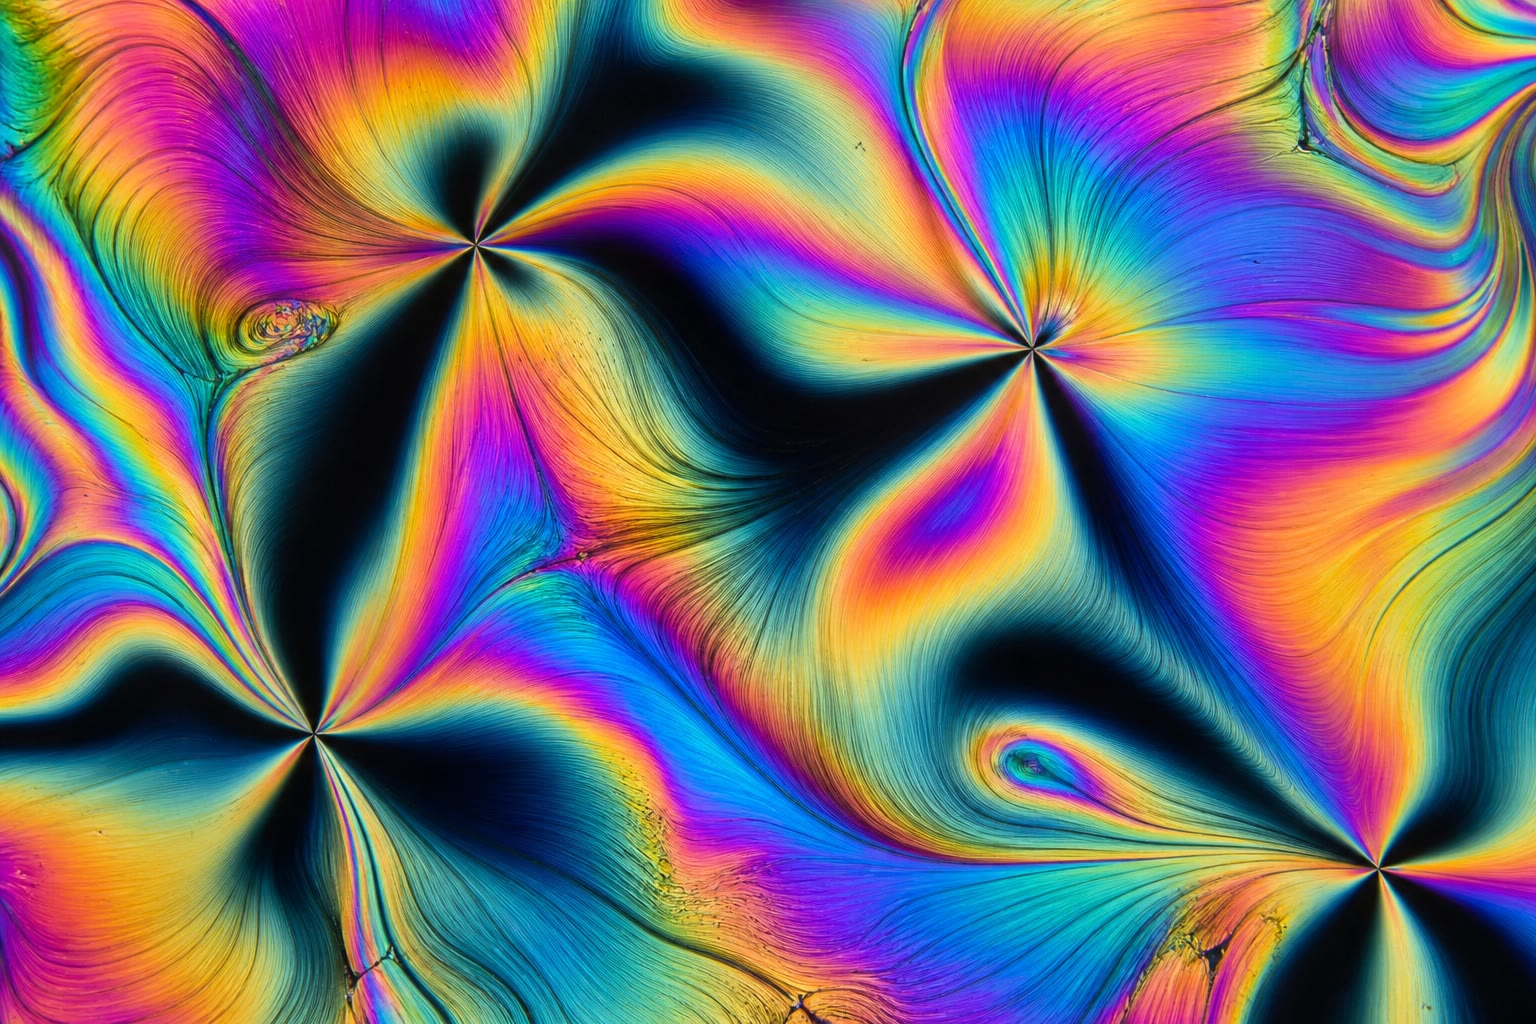
\includegraphics[width=0.58\linewidth]{images/book5/ai/b5-26-liquid-crystal.jpg}

{\small 正交偏振片之间的液晶：序参量（分子取向轴）在缺陷处盘旋，暗刷在此交汇。物质的相介于液体与固体之间，也是大多数屏幕的工作物质。}
\end{omfigure}

\section{练习}

\begin{exercise}[$\star$]\label{exo:b3:phase-transitions:1}
判断下列各情形属一级还是连续相变，并指明序参量
及所破缺的对称性（如有）：(a) \qty{1}{atm} 下的沸腾；(b)
居里点；(c) 超流体的 $\lambda$ 点；(d)
\emph{恰在}临界点处的沸腾。
\end{exercise}

\begin{exercise}[$\star$]\label{exo:b3:phase-transitions:2}
以熵表示潜热。(a) 水：$L_{\text{汽化}} =
\qty{2.26e6}{J/kg}$（\qty{373}{K}）下：求每个
分子的 $\Delta S$，以 $k_{\text{B}}$ 为单位。(b) 熔化的
同一量（$L_{\text{熔化}} = \qty{3.3e5}{J/kg}$，\qty{273}{K}）。(c) 多数
液体汽化时 $\Delta S \approx 10$--$11\,k_{\text{B}}$
（特鲁顿规则）：此数大致计数什么（取何种
体积比的 $\ln$）？(d) 为何熔化的熵跃变远小于
沸腾的？
\end{exercise}

\begin{exercise}[$\star$]\label{exo:b3:phase-transitions:3}
范德瓦耳斯临界常数（$V_{\text{c}} = 3Nb$，
$k_{\text{B}}T_{\text{c}} = 8a/27b$，$P_{\text{c}} = a/27b^2$——
可直接采用）。(a) 证明 $P_{\text{c}}V_{\text{c}}/Nk_{\text{B}}T_{\text{
c}} = 3/8$，为该模型的普适数；实测值
聚集在 $0.29$ 附近——请评论。(b) 对 CO$_2$
（$T_{\text{c}} = \qty{304}{K}$，$P_{\text{c}} = \qty{73.8}{bar}$）：
求出 $a$ 与 $b$。(c) 由 $b$ 估算分子
直径。(d) 为何室温下的 CO$_2$ 能在加压下液化，
而室温下的 N$_2$（$T_{\text{c}} =
\qty{126}{K}$）却从不液化？
\end{exercise}

\begin{exercise}[$\star$]\label{exo:b3:phase-transitions:4}
快速给出序参量：(a) 铁磁体；(b)
液–气转变；(c) 玻色–爱因斯坦凝聚；(d)
反铁磁体的序参量（两个子晶格——在总磁化强度
保持为零时，何种量有序？）。
\end{exercise}

\begin{exercise}[$\star\star$]\label{exo:b3:phase-transitions:5}
用手算平均场。(a) 由一个自旋推出 $m = \tanh(\beta qJm)$，
其平均场来自它的 $q$ 个近邻。(b) 证明非零
解恰在 $T < qJ/k_{\text{B}}$ 时存在。(c) 展开至
三阶，推出 $m(T) \approx \sqrt{3(1 -
T/T_{\text{c}})}$。(d) 铁：$T_{\text{c}} = \qty{1043}{K}$，$q =
8$：以电子伏特为单位求出 $J$，并核对
\cref{exo:b3:identical-particles:12}中的交换能标。
\end{exercise}

\begin{exercise}[$\star\star$]\label{exo:b3:phase-transitions:6}
居里–外斯。加入一个弱磁场：$m = \tanh[\beta(qJm + \mu B)]$。
(a) 在 $T_{\text{c}}$ 以上线性化，推出 $\chi = \partial
m/\partial B \propto 1/(T - T_{\text{c}})$。(b) 与自由自旋的居里定律相比较：
以 $1/\chi$ 对 $T$ 作图，在两种情形下
各得到什么，截距如何诊断铁磁
耦合？(c) 镍的 $1/\chi$ 直线在 \qty{631}{K} 处与零相交：
请解释。(d) 对反铁磁体，截距为
\emph{负}：这暴露了 $J$ 的何种符号？
\end{exercise}

\begin{exercise}[$\star\star$]\label{exo:b3:phase-transitions:7}
克劳修斯–克拉珀龙方程的应用。(a) \qty{100}{\celsius} 下的水
（$\Delta v = \qty{1.67}{m^3/kg}$）：计算 $\dd P/\dd T$。(b)
利用 $\dd\ln P/\dd T = Lm_{\text{w}}/k_{\text{B}}T^2$，估算
$P = \qty{0.7}{atm}$（海拔 \qty{3000}{m}
的山顶）下的沸点。(c) 熔化：取 $\Delta v = \qty{-9.1e-5}{m^3/kg}$ 与
$L = \qty{3.3e5}{J/kg}$，计算 $\dd T/\dd P$ 以及
使冰的熔点降低 \qty{5}{K} 所需的压强。(d) 一名
\qty{70}{kg} 的滑冰者站在 \qty{30}{mm^2} 的冰刀上：其压强及
熔点的变化量——压力熔化能否解释
滑冰？（真正起作用的是：摩擦力与表面预熔化。）
\end{exercise}

\begin{exercise}[$\star\star$]\label{exo:b3:phase-transitions:8}
朗道计算。(a) 极小化 $F = a(T - T_{\text{c}})m^2 +
bm^4$，温度在 $T_{\text{c}}$ 以下。(b) 计算极小值处的 $F$，并
证明热容在相变时有有限的\emph{跃变}，$\Delta C =
a^2T_{\text{c}}/2b$。(c) 画出 $C(T)$ 的示意图：
平均场给出阶跃，与之相对，氦的
$\lambda$ 点处实测为近对数型峰——真实涨落还增加了什么？(d)
加入场项 $-hm$：证明相变变得圆滑——
对称性必须严格成立，它才会破缺。
\end{exercise}

\begin{exercise}[$\star\star$]\label{exo:b3:phase-transitions:9}
成核。半径为 $r$ 的液滴处于过饱和蒸气中，
体相自由能减少 $-\tfrac43\pi r^3\,n\,\delta\mu$，但需付出
表面张力代价 $4\pi r^2\sigma$。(a) 证明势垒在
$r^* = 2\sigma/n\,\delta\mu$ 处达到峰值。(b) 解释：为何洁净的
过饱和蒸气与过热液体能够持续存在
（亚稳性），而尘埃、离子与划痕又起什么作用？
(c) 云室（\cref{ch:b3:particle-physics}中探测器的前身）与
气泡室正是\emph{基于}这一物理工作的：
飞越粒子留下的离子径迹起什么作用？(d) 实验室烧瓶中为何要放入
“沸石”？
\end{exercise}

\begin{exercise}[$\star\star\star$]\label{exo:b3:phase-transitions:10}
一维无相变。考虑由 $N$ 个自旋组成的一维伊辛链，
全部朝上，并引入一个“畴壁”（某一键之后的
所有自旋翻转）。(a) 畴壁的能量代价为 $2J$，
与位置无关。(b) 熵的增加：畴壁可位于
$\sim N$ 个键中的任一处——$\Delta S = k_{\text{B}}\ln N$。(c)
证明 $\Delta F = 2J - k_{\text{B}}T\ln N < 0$ 对任意 $T > 0$ 成立：
当 $N$ 很大时，畴壁总会大量增殖，长程序
不可能存在——一维伊辛模型的 $T_{\text{c}} = 0$。(d) 在
二维中，畴壁是长为 $\ell$ 的一条线，代价为 $2J\ell$，但
有 $\sim3^\ell$ 种形状：重新估计，并证明序
在有限的 $T_{\text{c}}$ 以下\emph{存续}——这正是
昂萨格精确解 $2.269\,J/k_{\text{B}}$ 背后的派尔斯论证。
\end{exercise}

\begin{exercise}[$\star\star\star$]\label{exo:b3:phase-transitions:11}
普适性审视。平均场预言 $\beta = 1/2$，$\gamma
= 1$（$\chi \sim |t|^{-\gamma}$），$\delta = 3$（$m \sim h^{1/3}$
于 $T_{\text{c}}$ 处）。实测结果，无论对液–气临界点
\emph{与}三维单轴磁体，均为 $\beta
\approx 0.326$，$\gamma \approx 1.237$，$\delta \approx 4.79$。
(a) 凭什么可以将流体与磁体相比较（它们的序参量有何共同之处——
唯一的符号选择）？(b)
为何平均场在 $T_{\text{c}}$ 附近失效（什么量发散，
从而使忽略涨落的做法不再成立）？(c) 为何它在
更高维度中\emph{较轻}地失效（近邻数目与涨落
作用范围之比较；平均场在四维以上精确成立）？
(d) 用两句话陈述重整化群的要旨：
逐尺度平均的是什么，以及为何只有
对称性与维数在平均之后得以保留。
\end{exercise}

\begin{exercise}[$\star\star\star$]\label{exo:b3:phase-transitions:12}
从磁体到希格斯。将序参量推广为场
$\phi(\vect r)$，其朗道能量密度为 $\alpha(T -
T_{\text{c}})\phi^2 + b\phi^4$ 加上梯度项。(a) 在 $T_{\text{c}}$ 以下
场取值为 $\pm\phi_0$：小振荡
\emph{沿}势阱的振荡具有回复曲率——计算
$F''(\phi_0)$，并用场论语言将其解释为
\emph{质量}。(b) 对\emph{复}序参量（极小值构成一个圆周——
“墨西哥帽”），\emph{绕}
边缘的振荡不需付出势能：这是一个无质量模式——请说出
其凝聚态类比（自旋波、超流声子）。(c)
在电弱理论中，真空本身位于这样一个
对称性破缺的势阱之中；粒子从场的
非零值获得质量，而径向振荡\emph{即是}希格斯
玻色子：将每个要素对应到 (a)–(b)。(d) 用一句话说明：
凝聚态物理在此为粒子物理提供了什么启示（
经由安德森输出的对称性破缺）？
\end{exercise}

\begin{omfigure}

\includegraphics[width=0.58\linewidth]{images/book5/ai/b5-17-pressure-cooker.jpg}

{\small 压力锅排气：内部两个大气压使液–气共存线移至 \qty{121}{\celsius}——克劳修斯与克拉珀龙，让晚餐烹饪得更快。}
\end{omfigure}

\section{问题：厨房中的相图}

\begin{problem}[{周末问题——压力锅、山上的
茶与沸腾的终结}]\label{pb:b3:phase-transitions:1}
水的相图悄然悬挂于每一个炉灶之上。本题
借助克劳修斯–克拉珀龙方程，逐一考察其三条曲线——
从压力锅为何能将烹饪时间减半，经由茶为何
在高海拔处令人失望，再到临界点以外那奇异的
世界，那里沸腾本身已不复存在。数据：$L_{\text{汽化}}
= \qty{2.26e6}{J/kg}$，$L_{\text{熔化}} = \qty{3.34e5}{J/kg}$；
水蒸气在 \qty{373}{K}、\qty{1}{atm} 下：$\Delta v_{\text{汽化}}
= \qty{1.67}{m^3/kg}$；熔化：$\Delta v = \qty{-9.1e-5}{m^3/kg}$；
分子质量 $m_{\text{w}} = \qty{3.0e-26}{kg}$；临界点：
$T_{\text{c}} = \qty{647}{K}$，$P_{\text{c}} = \qty{221}{bar}$。

\medskip\noindent\textbf{第一部分——沸腾线。}
\begin{enumerate}
  \item 在给定压强下，何为“沸腾”（由哪两个
        化学势相等来确定）？
  \item 计算汽化线的斜率 $\dd P/\dd T$
        （位于 \qty{100}{\celsius} 处）。
  \item 压力锅内压强为 \qty{2}{atm}：对斜率积分
        （或使用指数形式，并取 $Lm_{\text{w}}/
        k_{\text{B}} \approx \qty{4900}{K}$），求其沸点
        温度。
  \item 利用
        \cref{exo:b3:canonical-ensemble:9} 中的阿伦尼乌斯厨房规则（每
        \qty{10}{K}，反应速率加倍），估算相对于敞口锅
        烹饪的加速倍数。
  \item 在拉巴斯（\qty{3600}{m}，$P \approx \qty{0.65}{atm}$）：
        求沸点温度，并说明为何茶的冲泡效果不佳。
  \item 为何加盐会使沸点升高（溶质降低的是哪一个
        化学势 $\mu$——回顾
        \cref{exo:b3:grand-canonical:8}）？
\end{enumerate}

\medskip\noindent\textbf{第二部分——熔化线。}
\begin{enumerate}[resume]
  \item 计算熔化过程的 $\dd T/\dd P$，并注明其符号。
  \item 哪一种日常观察体现了 $\Delta v < 0$（冰块
        放在杯中会怎样），
        这种反常为何在物质中很少见？
  \item 一座厚 \qty{300}{m} 的冰川，其底部的压强
        与熔点降低量各为多少？底部压力熔化是否
        影响冰川的流动？
  \item 回顾 \cref{exo:b3:phase-transitions:7}(d) 中的滑冰者：
        究竟是什么
        在润滑冰刀？
  \item 若冰会下沉（斜率为正，与几乎所有其他固体一样），
        冬季将如何影响湖泊及其中的鱼类？
        请追踪这一连串的后果。
  \item 负斜率止于高压区，在那里其他冰的晶体形态接替
        出现（冰 III、V、VI）：
        十余种冰的存在，对一个简单
        分子的自由能图景说明了什么？
\end{enumerate}

\medskip\noindent\textbf{第三部分——线的终点。}
\begin{enumerate}[resume]
  \item 沸腾线终止于 ($T_{\text{c}},
        P_{\text{c}}$)：当趋近终点时，潜热与密度差
        将如何变化？
  \item 越过临界点后，可以使水从“类液态”变为“类气态”，
        而完全\emph{不}发生任何相变：在 $(P, T)$ 平面上
        描述这一路径。
  \item 接近临界点时，流体变得乳白：
        请将这种乳光现象与
        \cref{exo:b3:microcanonical-ensemble:12} 和
        \cref{pb:b3:perturbation-theory:1} 相联系。
  \item 超临界 CO$_2$（$T_{\text{c}} = \qty{304}{K}$，
        $P_{\text{c}} = \qty{74}{bar}$）像液体一样溶解，像气体一样渗透：
        请说出用于咖啡脱咖啡因的工业应用，
        并解释该溶剂为何不会留下
        残留物。
  \item 超临界水（在发电厂锅炉中压强高于 \qty{221}{bar}）：
        为何消除沸腾（气泡、气膜、烧毁）
        对锅炉工程师具有吸引力？
  \item 深海热液喷口喷出的水温为
        \qty{400}{\celsius} 却不沸腾：请对照当地
        压强（在 \qty{3}{km} 深处约 $\sim\qty{300}{bar}$）
        与相图进行检验。
\end{enumerate}

\medskip\noindent\textbf{第四部分——通读整张相图。}
\begin{enumerate}[resume]
  \item 用文字概述水的 $(P, T)$ 相图：三条曲线、
        三相点（$\qty{0.01}{\celsius}$，\qty{611}{Pa}）
        以及临界点。
  \item 在 \qty{611}{Pa} 以下，冰不经熔化直接升华：
        哪种设备（冷冻干燥）与哪颗行星的极冠
        （火星，CO$_2$ 与 H$_2$O）依赖于这一事实？
  \item 为何水的三相点——2019 年以前按定义恰为
        \qty{273.16}{K}——是如此好的温度标准
        （共存相的数目如何
        确定自由度的数目）？
  \item 相图中每条线都是一级相变，只有其端点
        是临界的：请用序参量与潜热
        重新表述这一区别。
  \item 潮湿空气的露点线是同一物理过程的逆向进行：
        请用一句涉及 $\mu$ 交叉的话，解释露水、雾，
        以及冷窗上的晨雾。
  \item 每个锅盖都是一个实验：水滴在其上凝结，
        又落回锅中——请指出这一微型水循环中的
        两种相变，以及使加盖锅更快沸腾的
        潜热往返传递。
  \item 总结这一著名结论：一个斜率公式 $\dd P/
        \dd T = L/T\Delta v$ 即可解释压力锅的
        \qty{121}{\celsius}、高山上 \qty{88}{\celsius} 的茶、
        冰沿其熔化线的反常走向而漂浮，以及
        超临界水壶：沸腾在
        $\qty{647}{K}, \qty{221}{bar}$ 处终止。
\end{enumerate}
\end{problem}
